\documentclass{beamer}
\usetheme{Berlin}
\usepackage[UTF8,scheme=plain]{ctex}
\usepackage{amsmath}
\usepackage{amsfonts}
\usepackage{amssymb}
\usepackage{mathrsfs}
\usepackage{bm}
\usepackage{graphicx}
\usepackage{float}
\usepackage{subfigure}
\usepackage{natbib}
\usepackage{graphicx}
\def\mathfamilydefault{\rmdefault}

\title{Measurement of the absolute branching fraction of the inclusive semileptonic $\Lambda_c^+$ decay}
\author{\kaishu{严启宇\ 黄吉鸿\ 卢玫澍}}
\institute{中国科学院大学, 北京}
\date{2019.07.25}

\begin{document}
\bibliographystyle{apalike}
\begin{frame}
    \titlepage
\end{frame}

\begin{frame}
    \frametitle{Outline}
    \tableofcontents
\end{frame}

\section{物理背景: 关于$\Lambda_c^+$}
\begin{frame}
    \sectionpage
\end{frame}

\begin{frame}
\indent $\Lambda_c^+$重子是含有charm夸克的重子中最轻的, 这一粒子在上世纪70年代年被发现. \cite{knapp1976observation},\cite{abrams1980observation}, 其夸克组分为udc. $\Lambda_c^+$有众多衰变路径, PDG上给出了现有的测量.\\
~\\
我们研究的\cite{ablikim2018measurement}是针对$\Lambda_c^+$的半轻衰变的合并分支比的测量. 此前人们对衰变$\Lambda_c^+ \rightarrow \Lambda e^+ \nu_e$的研究得到绝对分支比为$(3.63 \pm 0.43)\%$.\cite{ablikim2015measurement}. 
\end{frame}

\begin{frame}
然而1982年,MARK II合作组对衰变$\Lambda_c^+ \rightarrow X e^+ \nu_e$合并分支比的测量$(4.5 \pm 1.7)\%$对误差较大,这导致不能判断在这背后是否有未被发现的新的衰变模式. 于是, 准确的测定半轻衰变的分支比就是这篇文章的目的.\\
~\\
同时,这篇文章还要做的是测量半轻衰变$\Lambda_c^+\rightarrow\Lambda e^+\nu_e$占比
\begin{displaymath}
\frac{\mathcal{B}(\Lambda_c^+\rightarrow\Lambda e^+\nu_e)}{\mathcal{B}(\Lambda_c^+\rightarrow Xe^+\nu_e)}
\end{displaymath}
和与$D$半轻衰变$D\rightarrow Xe^+\nu_e$的衰变宽度比
\begin{displaymath}
\frac{\Gamma(\Lambda_c^+\rightarrow Xe^+\nu_e)}{\Gamma(D\rightarrow Xe^+\nu_e)}.
\end{displaymath}
\end{frame}

\section{实验方法}
\subsection{双标记法}
\begin{frame}
    \subsectionpage
\end{frame}

\begin{frame}
在本实验中利用了双标记法. 
\begin{figure}[h]
\centering
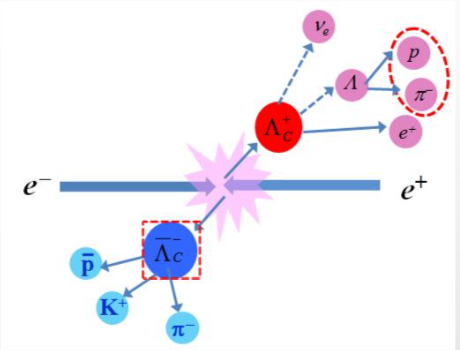
\includegraphics[scale=0.4]{DT.png}
\end{figure}
\end{frame}

\begin{frame}
关键: $\Lambda_c$永远成对产生, 所以重建了$n_1$个$\Lambda_c^-$, 其另一侧一定存在这$n_1$个$\Lambda_c^+$. 因此通过重建$\overline{\Lambda}_c^-\rightarrow\overline{p}K_s^0$和$\overline{\Lambda}_c^-\rightarrow\overline{p}K^+\pi^-$, 可以反推出$\Lambda_c^+$的数量. 再通过寻找电子$e^+$, 重建其半轻衰变, 这样就可以得到衰变分支比$\mathcal{B}(\Lambda_c^+\rightarrow Xe^+\nu_e)$.\\
~\\
近阈: 由于能量$\sqrt{s}=4.6\ \mathrm{GeV}$近阈, 所以没有更多的能量产生伴随的强子.

\end{frame}




\begin{frame}[allowframebreaks]
\bibliography{ref}
\end{frame}

\end{document}